\chapter{Algorithms}

In this section, we will go through several optimization algorithms and some bounds.

\section{Gradient Descent}
One of the most famous and frequently used optimization algorithms is the gradient descent, which can be formulated as:
\begin{equation}\label{eq:GradientDescentUpdateFormula}
    x_{k+1} \leftarrow x_k - \alpha_k\nabla f(x_k)
\end{equation}
Interestingly, this update formula can be interpreted in the following way:
\begin{equation*}
    x_{k+1} = \argmin_x \{ f(x_k) + \langle \nabla f(x_k), x-x_k \rangle + \frac{1}{2\alpha_k}\|x-x_k\|^2 \}
\end{equation*}
This means $x_{k+1}$ is the minimizer of the first-order approximation under quadratic distance penalty. In fact, if we denote $h(x) = f(x_k) + \langle \nabla f(x_k), x-x_k \rangle + \frac{1}{2\alpha_k}\|x-x_k\|^2$, by checking the first-order necessary condition, we have 
\begin{equation*}
    \nabla h(x) = \nabla f(x_k) + \frac{1}{\alpha_k}(x - x_k)
\end{equation*}
By setting $\nabla h(x) = 0$, we derive $x_{k+1} = x = x_k - \alpha_k\nabla f(x_k)$, which is the same as formula \ref{eq:GradientDescentUpdateFormula}.

\begin{note}
    One straightforward understanding of $\alpha_k$ is the step size taken as illustrated in \ref{eq:GradientDescentUpdateFormula}. However, as a quadratic in $h(x)$, it also represents how tolerant we are to distant condidates. Higher $\alpha_k$ indicates greater tolerance, corresponding to the gentler speed of change in the quadratic. 
\end{note}

Since we are interested in the minimization and maximization potential of the update algorithm, it's worth to explore how the corresponding value $f(x)$ changes. 
\begin{lemma}[Descent Lemma]\label{lemma:DescentLemma}
    Let $f: \mathbb{R}^d \rightarrow \mathbb{R}$ have L-Lipschitz gradient and $k \geq 0$, we have
    \begin{equation*}
        f(x_{k+1}) \leq f(x_k) - (\alpha_k - \frac{L\alpha_k^2}{2}) \| \nabla f(x_k) \|^2
    \end{equation*}
\end{lemma}
\begin{proof}
    Only need to use the first-order Taylor bound:
    \begin{equation*}
        | f(x_{k+1}) - f(x_k) - \langle \nabla f(x_k), x_{k+1} - x_k \rangle | \leq \frac{L}{2}\|x_{k+1} - x_k\|^2
    \end{equation*}
\end{proof}

\begin{corollary}
    If we take $\alpha_k = \frac{1}{L}$ as in exact linesearch, then we have:
    \begin{equation*}
        f(x_{k+1}) \leq f(x_k) - \frac{1}{2L} \| \nabla f(x_k) \|^2
    \end{equation*}
\end{corollary}

To minimize $f(x)$, we want the upper bound in lemma \ref{lemma:DescentLemma} to be as small as possible, meaning that we need to maximize $\alpha_k - \frac{L\alpha_k^2}{2}$. By solving this simple quadratic, we derive the ideal step size $\alpha_k = \frac{1}{L}$. However, this can be quite impractical since even if it's not a strong assumption to take functions we see in real life over a fintie domain as Lipschitz, it can be difficult to determine the Lipschitz constant $L$ for an unknown function. If we examine the update formula \ref{eq:GradientDescentUpdateFormula} closely, the only thing that needs external care is the step size $\alpha_k$. As a result, in the following we will discuss how to find a both effectively and pratically way to determine the step size $\alpha_k$.

\subsection{Exact Linesearch}

A straight forward approach is to find the solution of the following optimization problem, which is also referred to as the exact line search:
\begin{equation*}
    \alpha_k = \argmin_{\alpha \in \mathbb{R}}f(x_k - \alpha\nabla f(x_k))
\end{equation*}
Yet this can also be impractical because it means we have to solve an optimization problem at each step of update. In replacement to exact linesearch, we introduce the following backtracking linesearch algorithm by \emph{Larry Armijo}.

\subsection{Backtracking Linesearch}
The idea of backtracking linesearch is quite simple, we start with a step size large enough, and then shrink it little by little until we observe sufficient descent in $f(x)$. This can be formalized with the following two steps:
\begin{enumerate}
    \item Pick $\alpha \in \mathbb{R}_{>0}$ and $\tau \in (0,1)$, decrease step size by $\alpha_n = a\tau^n$.
    \item To measure the descent, we use the so-called Armijo condition.
\end{enumerate}
\begin{definition}[Armijo Condition]\label{def:ArmijoCondition}
    Pick $\eta \in (0,1)$, declare sufficient descent when 
    \begin{equation*}
        f(x_{k+1}) = f(x_k - \alpha\nabla f(x_k)) \leq f(x_k) - \eta\alpha\|\nabla f(x_k)\|^2
    \end{equation*}
\end{definition}

Therefore, we can restate the backtracking algorithm as:
\begin{equation*}
    \alpha_k = \max_n \{ a\tau^n : \text{Armijo condition holds for }\alpha = a\tau^n \}
\end{equation*}
One nice thing about Armijo's condition is that it clarifies the vague term "sufficient decsent". Beacuse we have $\eta \in (0,1)$, we certainly have the linear upper bound in \ref{def:ArmijoCondition} to be greater than $f(x - \alpha \cdot \nabla f(x))$ for $\alpha \in (0, \epsilon)$. One thing worth noticing is that, for $\eta$ small enough, it is possible for us to obtain multiple disconnected intervals with $\alpha$ satisfying the sufficient descent condition like $\eta = 0.3$.

\begin{figure}[H]
    \centering
    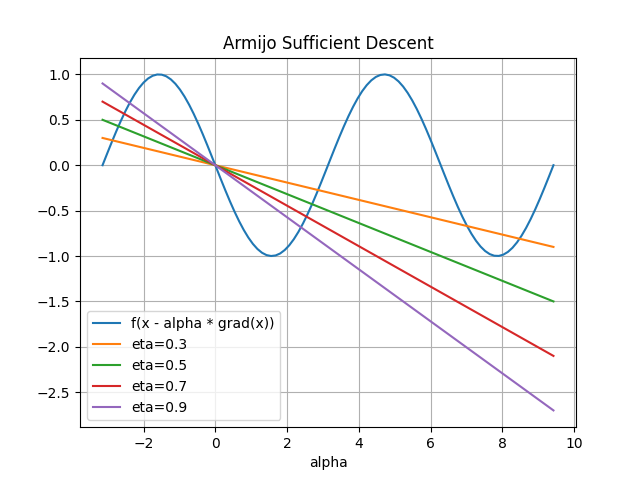
\includegraphics[scale=0.6]{plot_maker/Armijo_Sufficient_Descent/Armijo_sufficient_descent.png}
\end{figure}

Specifically, the following lemma describes the first Armijo interval near 0.

\begin{lemma}\label{lemma:ArmijoStepSizeBound}
    The Armijo condition holds for 
    \begin{equation*}
        \alpha \in [0, \frac{2(1 - \eta)}{L}]
    \end{equation*}
\end{lemma}
\begin{proof}
    Using the descent lemma, and bound the right hand side with linear upper bound, we have
    \begin{equation*}
        f(x_k - \alpha \nabla f(x_k)) \leq f(x_k) - (\alpha - \frac{L\alpha^2}{2})\|\nabla f(x_k)\|^2 \leq f(x_k) - \eta\alpha\|\nabla f(x_k) \|^2
    \end{equation*}
    This is the same as
    \begin{equation*}
        \eta\alpha \leq \alpha - \frac{L}{2}\alpha^2
    \end{equation*}
\end{proof}

\begin{note}[Consequences of Backtracking Linesearch]
    Firstly, in searching for step size $\alpha$, it needs no more than $\lceil \log_{\frac{1}{\tau}} (\frac{\alpha L}{2(1-\eta)}) \rceil $ steps to terminate. This bound is derived by asking $\alpha \tau^n \leq $ the bound in \ref{lemma:ArmijoStepSizeBound}. Secondly, we have $\alpha_k \geq \min\{ a, \frac{2\tau(1 - \eta)}{L} \}$ because we either find the sufficient descent at the first step, or find it no smaller than $\tau$ times the upper bound in \ref{lemma:ArmijoStepSizeBound}, which is the next iteration of step size. So we can rewrite the Armijo condition as:
    \begin{align}
        f(x_{k+1}) &\leq f(x_k) - \eta \alpha_k\|\nabla f(x_k) \|^2 \\
        &\leq f(x_k) - \eta \min\{ a, \frac{2\tau(1-\eta)}{L} \} \cdot \|\nabla f(x_k) \|^2  \label{eq:ArmijoUpdateBound}
    \end{align}
    Now in the special case where $a \geq \frac{1}{L}$ and $\eta = \tau = \frac{1}{2}$, we have 
    \begin{align*}
        (\ref{eq:ArmijoUpdateBound}) &\leq f(x_k) - \frac{1}{2}\min\{\frac{1}{L}, \frac{1}{2L}\} \cdot \|\nabla f(x_k) \|^2 \\
        &\leq f(x_k) - \frac{1}{4L}\| \nabla f(x_k) \|^2
    \end{align*}
    which does not result in a great sacrifice on the tightness of the bound compared with the quadratic in the descent lemma when the step size is small enough or asking $L > 1$. 
    
    A plot is available at \emph{Nonlinear\_Optimization/plot\_maker/Armijo\_and\_Descent\_Bound/plot.py}, python=3.11.5 + holoviews.
\end{note}

\section{NonConvex Smooth Optimization Guarantee}
Equipped with the bounding results on $f(x_{k+1})$ from the previous chapter, without convexity, we will see what we can say about L-smooth function and update rule:
\begin{equation*}
    x_{k+1} \leftarrow x_k - \alpha_k \nabla f(x_k)
\end{equation*}

\begin{theorem}[Bound on Average Gradient Norm for Nonconvex Functions]
    Suppose $f(x)$ is L-smooth, then for any $T > 0$, we have:
    \begin{equation*}
        \frac{1}{T}\sum_{k=0}^{T-1}\|\nabla f(x_k) \|^2 \leq \frac{2L}{T}(f(x_0) - \min_{0\leq k \leq T-1}f(x_k)) \leq \frac{2L}{T}(f(x_0) - \min_{x \in \mathbb{R}^d}f(x)) 
    \end{equation*}
    when we set $\alpha_k = \frac{1}{L}$, i.e. exact linesearch.

    In addition, with Armijo backtracking, we have:
    \begin{equation*}
        \frac{1}{T}\sum_{k=0}^{T-1}\|\nabla f(x_k) \|^2 \leq \frac{\max \{ \frac{1}{\eta a}, \frac{L}{2\tau\eta(1-\eta)} \}}{T}(f(x_0) - \min_{x \in \mathbb{R}^d}f(x))
    \end{equation*}
\end{theorem}
\begin{proof}
    Use the bound of $f(x_{k+1})$ we derived from the previous section, i.e. descent lemma \ref{lemma:DescentLemma} and Armijo. Sum all of the inequalities up, then change $f(x_k)$ to $\min f(x)$
\end{proof}

This theorem describes the average pattern of the sequence of the gradients $\{ \nabla f(x_k) \}$, it indicates that there exists at least one $x_k^*$ such that $\| \nabla f(x_k^*) \|$ itself satisfies the inequality. Now let's first define what is a second-order critial point, and then see what we can get if we enforce convexity on the function. 

\begin{definition}[Second-Order Critial Point]
    Given $f(x)$ twice differentiable, a point $x^* \in \mathbb{R}^d$ is said to be the critial point of $f(x)$ if we have 
    \begin{equation*}
        \nabla f(x^*) = 0 \text{ and } \nabla^2f(x^*) \succeq \lambda I_n, \;\exists \lambda > 0
    \end{equation*}
\end{definition}

\begin{theorem}
    Assume $f(x) : \mathbb{R}^d \rightarrow \mathbb{R}$ is twice differentiable and $x^*$ being its second-order critial point, and there exists $\epsilon > 0$, such that if $x_k \in B_\epsilon(x^*)$ then $x_l \in B_\epsilon(x^*),\;\forall l \geq k$. Then, if $x_0$ is close to $x^*$ we have:
    \begin{equation*}
        f(x_T) - f(x^*) \leq (1 - \frac{\lambda^2}{4L^2})(f(x_{T-1}) - f(x^*))
    \end{equation*}
\end{theorem}

This result has a strong implication, it means for functions with second-order critial points, or looser strongly convex functions, we have a quite fast(exponential) rate of approximation to the minimum. Because both $\lambda$ and $L$ are constant once $f(x)$ is settled.